

\tikzset{every picture/.style={line width=0.75pt}} %set default line width to 0.75pt        

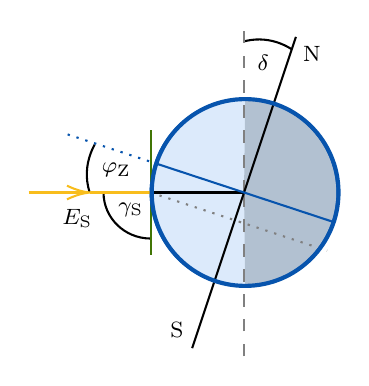
\begin{tikzpicture}[x=0.75pt,y=0.75pt,yscale=-1,xscale=1]
%uncomment if require: \path (0,181); %set diagram left start at 0, and has height of 181

%Shape: Arc [id:dp20953347708018688] 
\draw  [draw opacity=0] (69.43,111.09) .. controls (69.33,111.09) and (69.24,111.09) .. (69.15,111.09) .. controls (56.73,110.92) and (46.77,101.07) .. (46.73,89) -- (69.44,88.92) -- cycle ; \draw   (69.43,111.09) .. controls (69.33,111.09) and (69.24,111.09) .. (69.15,111.09) .. controls (56.73,110.92) and (46.77,101.07) .. (46.73,89) ;
%Shape: Arc [id:dp16591242877449974] 
\draw  [draw opacity=0] (40.06,88.92) .. controls (39.51,87.21) and (39.11,85.44) .. (38.89,83.61) .. controls (38.13,77.4) and (39.47,71.31) .. (42.46,65.81) -- (83.31,78.18) -- cycle ; \draw   (40.06,88.92) .. controls (39.51,87.21) and (39.11,85.44) .. (38.89,83.61) .. controls (38.13,77.4) and (39.47,71.31) .. (42.46,65.81) ;
%Straight Lines [id:da6013522376382066] 
\draw [color={rgb, 255:red, 65; green, 117; blue, 5 }  ,draw opacity=1 ]   (69.44,118.92) -- (69.44,88.92) ;
%Shape: Pie [id:dp028486029029515914] 
\draw  [color={rgb, 255:red, 0; green, 0; blue, 0 }  ,draw opacity=0 ][fill={rgb, 255:red, 0; green, 0; blue, 0 }  ,fill opacity=0.45 ] (114.95,43.91) .. controls (139.73,44.18) and (159.77,64.13) .. (159.85,88.77) .. controls (159.93,113.51) and (139.86,133.66) .. (114.94,133.93) -- (114.44,88.92) -- cycle ;
%Shape: Circle [id:dp7286185522053927] 
\draw  [color={rgb, 255:red, 7; green, 84; blue, 173 }  ,draw opacity=1 ][fill={rgb, 255:red, 200; green, 222; blue, 248 }  ,fill opacity=0.64 ][line width=0.75]  (69.44,88.92) .. controls (69.44,64.07) and (89.59,43.92) .. (114.44,43.92) .. controls (139.29,43.92) and (159.44,64.07) .. (159.44,88.92) .. controls (159.44,113.77) and (139.29,133.92) .. (114.44,133.92) .. controls (89.59,133.92) and (69.44,113.77) .. (69.44,88.92) -- cycle ;
%Shape: Arc [id:dp17913789171454497] 
\draw  [draw opacity=0] (114.15,16.18) .. controls (116.67,15.49) and (119.3,15.14) .. (121.99,15.17) .. controls (127.58,15.24) and (132.85,16.96) .. (137.52,19.97) -- (121.44,59.92) -- cycle ; \draw   (114.15,16.18) .. controls (116.67,15.49) and (119.3,15.14) .. (121.99,15.17) .. controls (127.58,15.24) and (132.85,16.96) .. (137.52,19.97) ;
%Straight Lines [id:da9967059081670446] 
\draw [color={rgb, 255:red, 128; green, 128; blue, 128 }  ,draw opacity=1 ] [dash pattern={on 4.5pt off 4.5pt}]  (114.44,167.84) -- (114.44,88.92) ;
%Straight Lines [id:da71597890822506] 
\draw [color={rgb, 255:red, 128; green, 128; blue, 128 }  ,draw opacity=1 ] [dash pattern={on 4.5pt off 4.5pt}]  (114.44,88.92) -- (114.44,10) ;
%Straight Lines [id:da4137878061890663] 
\draw [color={rgb, 255:red, 128; green, 128; blue, 128 }  ,draw opacity=1 ] [dash pattern={on 0.84pt off 2.51pt}]  (69.44,88.92) -- (111.94,102.92) ;
%Straight Lines [id:da3390187694217488] 
\draw [color={rgb, 255:red, 128; green, 128; blue, 128 }  ,draw opacity=1 ] [dash pattern={on 0.84pt off 2.51pt}]  (111.94,102.92) -- (154.44,116.92) ;
%Straight Lines [id:da5052190602488993] 
\draw    (114.44,88.92) -- (89.44,163.92) ;
%Straight Lines [id:da6983846735857875] 
\draw    (139.44,13.92) -- (114.44,88.92) ;
%Straight Lines [id:da5175201690882127] 
\draw    (69.44,88.92) -- (114.44,88.92) ;
%Straight Lines [id:da23163800871480023] 
\draw [color={rgb, 255:red, 65; green, 117; blue, 5 }  ,draw opacity=1 ]   (69.44,88.92) -- (69.44,58.92) ;
%Straight Lines [id:da47404926603772557] 
\draw [color={rgb, 255:red, 7; green, 84; blue, 173 }  ,draw opacity=1 ] [dash pattern={on 0.84pt off 2.51pt}]  (29.44,60.92) -- (71.94,74.92) ;
%Straight Lines [id:da6548182479176137] 
\draw [color={rgb, 255:red, 248; green, 189; blue, 28 }  ,draw opacity=1 ]   (10.69,88.92) -- (38.06,88.92) ;
\draw [shift={(40.06,88.92)}, rotate = 180] [color={rgb, 255:red, 248; green, 189; blue, 28 }  ,draw opacity=1 ][line width=0.75]    (10.93,-3.29) .. controls (6.95,-1.4) and (3.31,-0.3) .. (0,0) .. controls (3.31,0.3) and (6.95,1.4) .. (10.93,3.29)   ;
%Straight Lines [id:da7518207882403078] 
\draw [color={rgb, 255:red, 248; green, 189; blue, 28 }  ,draw opacity=1 ]   (40.06,88.92) -- (69.44,88.92) ;
%Shape: Circle [id:dp4417291051670942] 
\draw  [color={rgb, 255:red, 7; green, 84; blue, 173 }  ,draw opacity=1 ][fill={rgb, 255:red, 200; green, 222; blue, 248 }  ,fill opacity=0 ][line width=1.5]  (69.95,88.91) .. controls (69.95,64.06) and (90.1,43.91) .. (114.95,43.91) .. controls (139.8,43.91) and (159.95,64.06) .. (159.95,88.91) .. controls (159.95,113.77) and (139.8,133.91) .. (114.95,133.91) .. controls (90.1,133.91) and (69.95,113.77) .. (69.95,88.91) -- cycle ;
%Straight Lines [id:da09584357360735729] 
\draw [color={rgb, 255:red, 7; green, 84; blue, 173 }  ,draw opacity=1 ]   (71.94,74.92) -- (114.44,88.92) ;
%Straight Lines [id:da1322107965109387] 
\draw [color={rgb, 255:red, 7; green, 84; blue, 173 }  ,draw opacity=1 ]   (114.44,88.92) -- (156.94,102.92) ;

% Text Node
\draw (44.44,73.32) node [anchor=north west][inner sep=0.75pt]  [font=\footnotesize]  {$\varphi _{\mathrm{Z}}$};
% Text Node
\draw (119.44,21.32) node [anchor=north west][inner sep=0.75pt]  [font=\footnotesize]  {$\delta $};
% Text Node
\draw (25.44,95.4) node [anchor=north west][inner sep=0.75pt]  [font=\footnotesize]  {$E_{\mathrm{S}}$};
% Text Node
\draw (141.44,16.92) node [anchor=north west][inner sep=0.75pt]  [font=\footnotesize] [align=left] {N};
% Text Node
\draw (77.44,149.92) node [anchor=north west][inner sep=0.75pt]  [font=\footnotesize] [align=left] {S};
% Text Node
\draw (52.44,92.32) node [anchor=north west][inner sep=0.75pt]  [font=\footnotesize]  {$\gamma _{\mathrm{S}}$};


\end{tikzpicture}
